\documentclass[aspectratio=169]{beamer}
\usepackage{cmlgc}%шрифт
\usepackage[T2A]{fontenc}
\usepackage[utf8]{inputenc}
\usepackage[english,russian]{babel}
\usepackage{color}
\definecolor{GreenYellow}{RGB}{173,255,47}%{204,255,0}лайм
\graphicspath{{images/}}
\usepackage{wrapfig}
\setbeamertemplate{navigation symbols}{}% отключить клавиши навигации

\newcommand{\blu}{\textcolor{blue}}
\newcommand{\zag}{\huge\alert}
\newcommand{\n}{\normalsize}

\usetheme{Dresden}% тема
\usecolortheme{crane}% {beaver}%красная цветовая схема

\title{Билет №8}
\subtitle{1.Представление звуковой и видео информации. Форматы звуковых и видео файлов.\\ 2.Булева алгебра, постулаты(аксиомы) булевой алгебры.}

\author{\small студент группы 8871\\ Храпов Михаил} 
\institute{\scriptsize СПБГЭУ «ЛЭТИ» им. В.И. Ульянова (Ленина)}
\date{\today} 
% \logo{\includegraphics[height=5mm]{/Bg.png}\vspace{-7pt}}
\setbeamercolor{normal text}{bg=GreenYellow}%Background документа
\begin{document}

% титульный слайд
\begin{frame}
\titlepage
\end{frame} 
%%%%%%%%%%%%%%%%%%%%%%%%%%%%%%%%%%%%%%%%%%%%%

\section{Аудио и видео. Форматы}
\begin{frame}{Звуковая и видео информация.Восприятие человеком}

\framesubtitle{Тема №1}

\begin{columns}
\begin{column}[t]{7cm}
\small Воспринемаемые человеком \textbf{звуковые волны} представляют собой механические колебания окружающей среды различной амплитуды и с частотой варьирующейся в диапазоне от 20 до 20000 Гц, преобразуемые внутренним ухом в нервные импульсы.\\ 
\begin{figure}[h!]
\centering
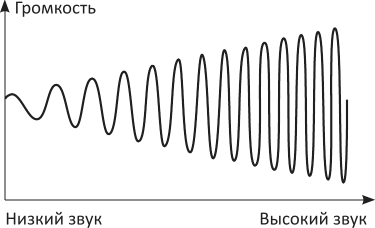
\includegraphics[width=4cm]{sound.png}
\end{figure}
\end{column}
\begin{column}[t]{7cm}
\small Визуальная-же информация это \textbf{поток фотонов} излучаемый или отражаемый обьектами, попадающий через глазное яблоко на слой светочуствительных рецепторов. Рецепторы раскладывают поток на световую и цветовую составляющие, и преобразуют его всё в те-же нервные импульсы.
\begin{figure}[h!]
\centering
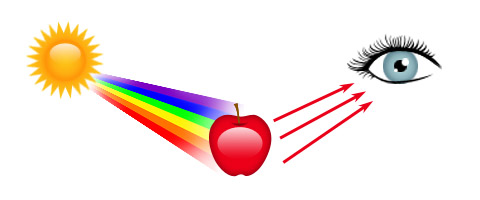
\includegraphics[width=4cm]{vi.jpeg}
\end{figure}
\end{column}
\end{columns}
\end{frame}
%%%%%%%%%%%%%%%%%%%%%%%%%%%%%%%%%%%%%%%%%%%%%
\begin{frame}
\frametitle{Аналоговый звук} 
Для начала разберёмся со звуком: как мы можем хранить и воспроизводить подобного вида информацию? Ведь сохранить звуковую волну в "сыром" виде не получится. Решением этой проблемы стало преобразование механических колебаний в колебания иного рода. Первыми "полноценными" носителями звуковой информации явились магнитные ленты и виниловые пластинки.
\begin{wrapfigure}{r}{0.27\linewidth}
\vspace{-1ex}%сдвиг вверх
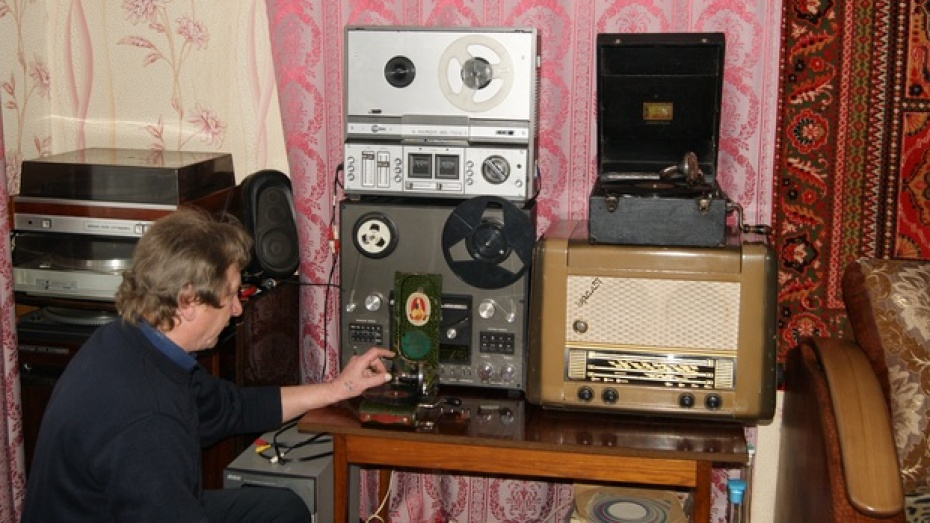
\includegraphics[width=4.1cm]{analog.jpeg}
\end{wrapfigure} 
Звуковая волна на таких носителях\\ сохраняется в виде непрерывного электрического сигнала, определяющего изменение звуковых волн. Такой метод записи, модулирующий изначальную волну называется \textbf{аналоговым}.

\end{frame}
%%%%%%%%%%%%%%%%%%%%%%%%%%%%%%%%%%%%%%%%%%%%%
\begin{frame}{Аналоговое видео}
    Кодировать световой поток в последовательность электрических сигналов, несущих информацию о яркости и цвете отдельных участков изображения, приемлимую для записи на магнитную ленту стало возможным после изобретения "электронно-лучевой трубки".{\ttfamily {\footnotesize \blu{ *На самом деле были предшественники и у бобины с электронно-лучевой трубкой. Звук успешно записывали при помощи цилиндров с выступами(как в шарманках, музыкальных шкатулках или в гидравлических органах) или же перфорированых бумажных карт(для пианол). История видео так-же уходит корнями в аппарат Бейна(который был способен передавать изображения по телеграфной линии) и  диск Нипкова (электро-механический прибор, лёгший в основу механического телевидения). Но все эти устройства и методы, на мой взгляд, ещё слишком далеки от понятия "информации" в современной интерпритации.}}}
\end{frame}
%%%%%%%%%%%%%%%%%%%%%%%%%%%%%%%%%%%%%%%%%%%%%
\begin{frame}{Переход к "цифре"}

    \footnotesize По мере развития ЭВМ становилось очевидно что аудио/видео необходимо адаптировать для хранения и использования в цифровой среде.
    \begin{columns}
\begin{column}[t]{6.9cm}
\alert{Аналогово-цифровое преобразование сигнала состоит из 3-х этапов}
\begin{itemize}
    \item \blu{Дискретизации} – \scriptsize представления непрерывного сигнала в виде последовательного набора отдельных амплитуд(мнгновенных значений)
    \item \n \blu{Квантования} – \scriptsize разделения каждой амплитуды на заданное число уровней
    \item \n \blu{Кодирования} – \scriptsize записи данных позиции и уровня амплитуды в цифровом виде.
\end{itemize}
В случае звука эти преобразования выполняются устройствами называемыми АЦП или ЦАП. Количество бит, отводимое на один звуковой сигнал, называют \textbf{ глубиной кодирования звука.}
\end{column}
\begin{column}[t]{7cm}
\alert{К видео применяется термин "захват" (англ. Video capture)}\\
"Захват" может производиться как с аналогового источника (т.н."оцифровка") либо, как в случае с DV-источниками, изначально сжатый цифровой видеопоток может передаваться от видеоисточника на компьютер. Например при помощи интерфейса IEEE 1394.
 \begin{figure}[h]
  \begin{minipage}[h]{0.47\linewidth}
  \center{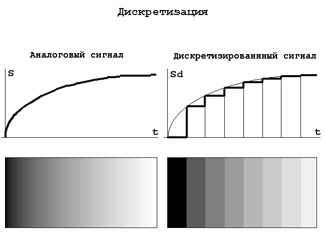
\includegraphics[width=2.6cm]{diskr.jpg}}
  \end{minipage}
  \begin{minipage}[h]{0.47\linewidth}
  \center{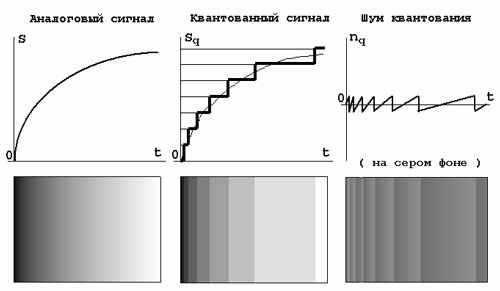
\includegraphics[width=3.45cm]{qwant.jpg}}
  \vspace{-2ex}
  \end{minipage}
 \end{figure}
\end{column}
\end{columns}
\end{frame}
%%%%%%%%%%%%%%%%%%%%%%%%%%%%%%%%%%%%%%%%%%%%%
\begin{frame}[shrink=11]{Подробнее о кодировании}

 \alert{Дискретизация \scriptsize (Процесс замены непрерывного сигнала дискретным, то есть превращение его в последовательность электрических импульсов (двоичных нулей и единиц)).}\\ \footnotesize   Она состоит из 2ух параметров. 
   \begin{itemize}      
         \item  \textbf{частота дискретизации}, отвечающая за качество звука, и варьирующаяся в диапазоне \textbf{от 8 до 48кГц}(\blu{48кГц-стандарт аудиоCD.В настоящее время частота может достигать гораздо больших величин}) Иначе - количество измерений \textbf{громкости} звука за одну секунду
         \item  \textbf{глубина дискретизации} (количество информации, которое необходимо для кодирования дискретных уровней громкости цифрового звука.)
    \end{itemize}
    *Если известна глубина кодирования, то количество уровней громкости цифрового звука можно рассчитать по формуле $N = 2^I$, а современные звуковые карты обеспечивают  16, 32 или  64 битную глубину кодирования.

\vspace{10pt}

    Необходимо помнить, что чем выше качество цифрового звука, тем больше информационный объем звукового файла.
    
    
Оценить информационный объём \alert{моно}аудиофайла $V$ можно по формуле \alert{$V=N\cdot f\cdot k$}, где  $N$  — общая длительность звучания (секунд),  $f$  — частота дискретизации (Гц),  $k$  — глубина кодирования (бит). А при кодировании \alert{стерео}звука дискретизация происходит отдельно для правого и левого каналов, что в итоге \alert{удваивает} обьём файла.
    
\end{frame}
%%%%%%%%%%%%%%%%%%%%%%%%%%%%%%%%%%%%%%%%%%%%%
\begin{frame}[shrink=11]{"Масса" проблем}

"Оцифровка", особенно на заре компьютеростроения, сталкнулась с серьёзной проблемой. В то время как ёмкость носителей доходила до нескольких десятков Мбайт, аудио, и в особенности видео в базовых форматах занимали чудовищно много места.Кадр видео аналогового формата \alert{PAL}(англ. Phase Alternating Line — построчное изменение фазы) состоит из  720  точек по горизонтали и  576  по вертикали. То есть один кадр состоит из  414720  точек.
Для хранения цвета каждой точки в памяти отводится  24  бита (по  8  бит для каждой из составляющих RGB).
Следовательно, для хранения одного кадра понадобится  9953280  бит (или примерно  1,2  Мбайт).
То есть секунда несжатого видео в формате PAL будет занимать почти  30  Мбайт. А один час такого видео — более  100 Гбайт!

\vspace{10pt}

Решением этой проблемы стало \alert{"сжатие"} - применение специальных алгоритмов для удаления из аудио/видео "лишних" элементов, основаная на особенностях и дефектах человеческого восприятия. Применение сжатия позволило сократить объёмы файлов в десятки, а то и сотни раз, но по большей части приводило к необратимой потере информации (данные не могут быть восстановлены в первоначальном виде).
\end{frame}
%%%%%%%%%%%%%%%%%%%%%%%%%%%%%%%%%%%%%%%%%%%%%
\begin{frame}{Кодировать, раскодировать...}% минутка юмора -_-'

    Вот и получается, что изначальные звуковые и свето-цветовые волны закодированы в последовательности единиц и нулей, сжаты, и лежат себе, хранятся. И тут мы решаем взять и проиграть то что мы там записали. И опять встаёт вопрос: Как? Как мы можем воспринять эту информацию? И казалось-бы, всё же прекрасно складывается. Тут электонные сигналы, и в голове электронные сигналы! Бери да передавай... эээ, не тут то было. Не дошёл ещё прогресс до таких технологий. А значит надо всю эту морзянку что?.. правильно! Возвращать к \alert{аналоговому} виду.
    
    \vspace{10pt}
    
    Тут мы и подходим к понятию \alert{кодек}(\footnotesize абр. от КОмпрессор и ДЕКодер), \n тесно связаному с форматами. Но об этом позже.
\end{frame}
%%%%%%%%%%%%%%%%%%%%%%%%%%%%%%%%%%%%%%%%%%%%%
\begin{frame}[shrink=5]{Добрались и до форматов}%Ура!

Форматы.. Что это такое?.\\ Понятие формат\footnotesize \blu{(от нем. format, фр. format < лат. forma — наружность)} \n довольно широко. В него входят \textit{\textbf{как}} структура и особенности представления данных в медиа\alert{файлах} (хранящихся ячейках информации), или, например, в \alert{видеопотоках} (не являющихся хранимыми единицами информации), \textit{\textbf{так}} и более широкие понятия (формат носителя, алгоритм кодирования и сжатия, телевизионные вещательные стандарты и др.)

\begin{wrapfigure}{r}{0.35\linewidth}
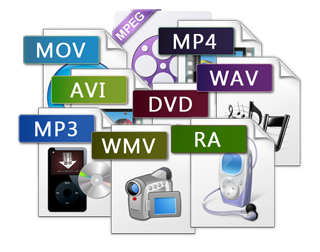
\includegraphics[width=4cm]{format.png}
\end{wrapfigure}

Интересующее нас понятие формат включает:

\begin{itemize}
\setlength\itemsep{2mm}
    \item \small Представление аудио данных
    \item Представление видео данных
    \item Кодеки(\scriptsize\blu{для одних форматов определён однозначно,\\ для других может варьироваться})
    \item \nМедиаконтейнеры(\scriptsize\blu{В них могут содержаться аудио/видео сжатые различными комбинациями кодирования})
\end{itemize}
\end{frame}
%%%%%%%%%%%%%%%%%%%%%%%%%%%%%%%%%%%%%%%%%%%%%
\begin{frame}[shrink=15]{Общие данные}

    Насчитывается около сотни форматов звука и ещё больше форматов видео, и их список постоянно пополняется! По мере разработки новых технологий позволяющих ещё лучше сжать, ускорить процесс обработки или же улучшить качество по сравнению с предшественниками, появляются новые форматы. Приводить их полный список будет очень сложно и долго. А по сему мы определим \alert{основные категории форматов и их отличительные особенности}. Ну а подробно рассмотрим только некоторые из них.
    \vspace{12pt}
    \begin{columns}[t]
    \begin{column}{5.55cm}
\blu{\textbf{Форматы аудио}}
\begin{itemize}
    \item без сжатия(\alert{WAW,AIFF})
    \item со сжатием без потерь(\alert{APE,FLAC,ALAC})
    \item со сжатием с потерями (\alert{MP3, Ogg})
\end{itemize}
    \end{column}
    
\vrule{}
    
    \begin{column}{6.55cm}
\blu{\textbf{Форматы видео}}

\alert{практически тождественны контейнерам} \small=> как правило, уже содержат в себе аудио. Классифицировать алгоритмы кодирования видео мы не будем, т.к. они очень сложны и их подробные описания можно найти только в специальной литературе. По этому мы рассмотрим их в составе \alert{контейнеров}.
    \end{column}
    
\vrule{}
    
    \begin{column}{6.6cm}
\blu{\textbf{Специфические форматы}}

Такой формат звука как \alert{MIDI} представляет собой протокол\\ передачи музыкальных нот и\\ мелодий. Но его данные не являются цифровым звуком - это сокращенная форма записи музыки в числовой форме.
    \end{column}
\end{columns}
\end{frame}
%%%%%%%%%%%%%%%%%%%%%%%%%%%%%%%%%%%%%%%%%%%%%
\begin{frame}[shrink=32]{Основные форматы видео файлов}


    \zag{MPEG}\n (\textbf{*.MPG, *.MPEG}) - формат для записи и воспроизведения видео. Имеет собственный алгоритм компрессии. В настоящее время активно используются для записи цифрового видео. Наиболее широкое распространение нашли два формата: \alert{MPEG-1} и \alert{MPEG-2}. Они различаются по объему и качеству получаемой видеоинформации и признаны междуна­родными стандартами для сжатия видео. В настоящее время наряду с \alert{MPEG-1} и \alert{MPEG-2} используется формат \alert{MPEG-4}. Он позволяет сжать информацию с большим коэффициентом.
    
    \vspace{10pt}
 
    \zag{AVI}\n \textbf{(Audio-Video Interleaved; букв. "чередование аудио и видео")} - один из самых распространенных медиаконтейнеров для ОС Windows. Этот формат может содержать в себе информацию четырех типов: видео, аудио, текст и \alert{midi}. В него может входить видео различных форматов: несжатое видео, видео в форматах \alert{DV}, MPEG-4, DivX, Xvid и даже MPEG-1 и MPEG-2. Кроме того, файл формата AVI может, например, содержать в себе только звук. Медиаконтейнер \alert{AVI} не накладывает никаких ограничений на тип используемых кодеков. (\blu{Следующим Microsoft'овским приемником стал} \alert{WMV}.)
    
    \vspace{10pt}
    
    \zag{MOV}\n - этот формат разработан компанией Apple для \textbf{QuickTime} медиа плеера. Формат может содержать видео, анимацию, графику, 3D. Данный формат поддерживает любые аудио- и видеокодеки.
    
    \vspace{10pt}
    
    \zag{FLV}\n (\textbf{Flash Video}) — формат файлов, медиаконтейнер, используемый для передачи видео через Интернет. Используется такими сервисами видеохостинга как YouTube, Google Video, Вконтакте, RuTube и другими. Хотя описание формата контейнера было открыто, кодеки защищены патентами.

\end{frame}
%%%%%%%%%%%%%%%%%%%%%%%%%%%%%%%%%%%%%%%%%%%%%
\begin{frame}[shrink=24]{Чуть подробней про MPEG}

    \zag{MPEG}\n (англ.\textbf{Moving Picture Expert Group}) \textbf{"Экспертная группа по движущимся изображениям"} - международная организация по стандартизации (\textbf{ISO}), впервые собравшаяся в мае 1988 года в Оттаве, и в \textbf{1992г.} явившая миру первый стандарт \alert{MPEG-1}.
    
    \vspace{5pt}
    
    За время своего существования группа произвела:
    \begin{itemize}
\setlength\itemsep{1mm}
        \item \alert{MPEG-1}: Исходный стандарт сжатия видео и аудио. Позднее использовался как стандарт для \blu{Video CD}.
        \item \alert{MPEG-2}: Транспортные, видео- и аудиостандарты для широковещательного телевидения. Используется в цифровом телевидении \blu{ATSC}, \blu{DVB} и \blu{ISDB}, цифровых спутниковых ТВ-службах, таких как \blu{Dish Network}, цифровом кабельном телевидении и (с небольшими изменениями) в \blu{DVD}.
        \item \alert{MPEG-3}: Изначально разрабатывался для \blu{HDTV}, но был отвергнут, когда обнаружилось, что для него вполне достаточно \blu{MPEG-2} (с расширениями).
        \item \alert{MPEG-4}: Расширение \blu{MPEG-1} для поддержки «объектов» видео/аудио, 3D-контента, сжатия с низким битрейтом и \blu{DRM}.%защита авторских прав
        В него включено несколько новых высокоэффективных видеостандартов таких как: \blu{MPEG-4 Part 2 (ASP)} и
\blu{MPEG-4 Part 10} (\blu{также известный как H.264 или AVC}). \blu{MPEG-4 Part 10} используется в дисках \blu{HD DVD} и \blu{Blu-ray}.
    \end{itemize}

\vspace{10pt}

\small Так-же в их арсенале имеется стандарт \alert{MPEG-7} посвящённый индексации мультимедиа содержимого, и находящийся в разработке долговременный проект \alert{MPEG-21}, описываемый разработчиком как "мультимедийная среда разработки".
\end{frame}
%%%%%%%%%%%%%%%%%%%%%%%%%%%%%%%%%%%%%%%%%%%%%
\begin{frame}[shrink=31]{Основные форматы звуковых файлов}


    \zag{WAVE}, \nили \zag{WAV}\n, (от англ. \textbf{waveform} — "в форме волны") — формат файла-контейнера для хранения записи оцифрованного аудиопотока, подвид \alert{RIFF}(\textbf{Resource Interchange File Format}). Обычно используется для хранения несжатых аудио-записей (\alert{PCM}), идентичных по качеству звука записям на компакт-дисках (\alert{audio-CD}). В среднем одна минута звука в формате wav занимает около 10 мегабайт.

 \vspace{10pt}
 
 \zag{FLAC}\n – популярный формат сжатия без потерь. Он не вносит изменений в аудио-поток и закодированный с его помощью звук идентичен оригиналу. Часто используеется для прослушивания звука на звуковых системах высокого уровня. Имеет огранченную поддержику устройствами и плеерами, поэтому обычно для того, чтобы слушать \alert{flac} в плеере, его предварительно конвертируют.
 
 \vspace{10pt}
 
 \zag{AAC}\n (\textbf{Advanced Audio Coding})  – запатентованный аудио-формат, имеющий б\'{о}льшие возможности (количество каналов, частоты дискретизации)  в сравнении с mp3, и дающий несколько лучшее звучание при том же размере файла. На данный момент \alert{aac} является одним из самых качественных алгоритмов кодирования звука с потерями. Формат поддерживается большинством устройств. Файл этого формата может иметь расширения \alert{aac, mp4, m4a, m4b, m4p, m4r}.
 
  \vspace{10pt}
 
 \zag{OGG}\n – открытый формат, поддерживающий кодирование аудио различными кодеками. Наиболее часто в \alert{ogg} используется кодек \alert{Vorbis}. По качеству сжатия формат сопоставим с \alert{MP3}, но при этом менее распространен с точки зрения поддержки в аудио-проигрывателях и плеерах.
 
 \end{frame}

\begin{frame}[shrink=28]{И на десерт..}
\framesubtitle{Конец первой темы}
     \zag{MP3}\n (\textbf{MPEG-1/2/2.5 Layer 3}) - самый распространённый (и поддерживаемый проигрывателями) формат "сжатого аудио с потерями" по сей день. Хотя сейчас существуют форматы сжимающие звук сильнее и с лучшим качеством (тот-же \alert{AAC}), огромная распространённость не даёт \alert{MP3} кануть в лету. Алгоритмы сжатия у \alert{MP3} и его последователей основаны на одинаковых принципах, и по этому имеет смысл разобрать его подробней.
     \begin{itemize}
         \item Аудиосигнал разбивается на \blu{фреймы} (короткие срезы волны), и над каждым из них производится \blu{дискретное преобразование Фурье}(Разложение сигнала на составляющие его частоты, и запись их амплитуд). Так-же срезаются все сигналы частотой выше 16000Гц.
         
         \item Далее применяется \blu{эффект маскировки}, состоящий из \blu{частотной} (\textit{эффект "заглушения" сигналом с большой амплитудой соседних частот и частот кратных ему (\blu{гармоник}})) и \blu{временной} (\textit{Кратковременный период "глухоты" человека сразу после воздействия громких звуков (\approx 0.05с}))
         
         \item Далее (в случае стерео) каналы записываются в форме $\frac{L+R}{2}$ и $L-R$. Это обусловлено сравнительно малым количеством отличий в звучании разных каналов по отношению друг к другу, и позволяет более грубо кодировать их разность.
         
         \item После чего файл прогоняют через "алгоритм \blu{Хаффмана}" - наиболее часто встречающиеся последовательности (\textit{та же удалённая предыдущими процедурами информация}) кодируются коротким кодом в несколько бит.
         
         \item В заключении, оставшиеся после обработки коэффициенты преобразования фурье записываются в фреймы и склеиваются в готовый \alert{MP3}-файл.
     \end{itemize}
\end{frame}
%%%%%%%%%%%%%%%Конец первой части%%%%%%%%%%%%%%%%%%
\section{Булева алгебра и её аксиомы}
\begin{frame}{Булева алгебра. Логические высказывания.}
\framesubtitle{Тема №2}
    \begin{wrapfigure}{r}{0.09\linewidth}
\vspace{-2em}%сдвиг вверх
    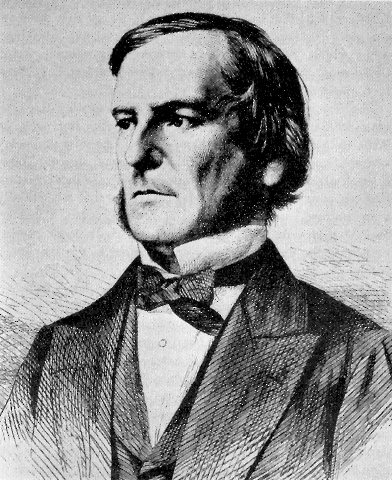
\includegraphics[width=2cm]{george.jpg}
    
    \scriptsize Джордж Буль
    \end{wrapfigure}

     \zag{Булева алгебра} \n(известная как \blu{алгебра логики}) - это раздел математики, изучающий \alert{высказывания} со стороны их логических значений\\ и логические операции над ними.\\
        \vspace{10pt}
    \alert{Логическое высказывание} - это любое повествовательное предложение, в отношении которого можно \alert{однозначно!} сказать \alert{Истинно} оно или \alert{Ложно}\\
    \vspace{10pt}
    
\begin{exampleblock}{Пример}
    \footnotesize 
    \textit{Предложение \textbf{"Трава зеленая"} следует считать высказыванием, так как оно \alert{истинное}.}

\textit{Предложение \textbf{"Конь - самолёт"} тоже высказывание, так как оно \alert{ложное}.}
\end{exampleblock}

\end{frame}
%%%%%%%%%%%%%%%%%%%%%%%%%%%%%%%%%%%%%%%%%%%%%
\begin{frame}[shrink=20]{Логические связки}

Употребляемые в обычной речи слова и словосочетания \alert{"не"}, \alert{"и"}, \alert{"или"}, \alert{"если... , то"}, \alert{"тогда и только тогда"} и другие позволяют из уже заданных высказываний строить новые высказывания. Такие слова и словосочетания называются \blu{Логическими связками}.\\
\vspace{10pt}
Bысказывания, образованные из других высказываний с помощью \blu{логических связок}, называются \alert{составными}. Высказывания, не являющиеся составными, называются  \alert{элементарными}.
\begin{exampleblock}{"и"}
    \textit{Из элементарных высказываний \textbf{"Петров — врач"}, \textbf{"Петров — шахматист"} при помощи связки \alert{"и"} можно получить составное высказывание \textbf{"Петров — врач и шахматист"}, понимаемое как \textbf{"Петров — врач, хорошо играющий в шахматы"}.}
\end{exampleblock}
\begin{exampleblock}{"или"}
\textit{При помощи связки \alert{"или"} из этих же высказываний можно получить составное высказывание \textbf{"Петров — врач или шахматист"}, понимаемое в алгебре логики как \textbf{"Петров или врач, или шахматист, или и врач и шахматист одновременно"}}.
\end{exampleblock}
    
\end{frame}
%%%%%%%%%%%%%%%%%%%%%%%%%%%%%%%%%%%%%%%%%%%%%
\begin{frame}{Логические связки}
Чтобы обращаться к логическим высказываниям, им назначают имена.
\begin{exampleblock}{Пример}
\textit{Пусть через \alert{А} обозначено высказывание \textbf{"Тимур поедет летом на море"}, а через \alert{В} — высказывание \textbf{"Тимур летом отправится в горы"}.}

\vspace{10pt}

\textit{Тогда составное высказывание   \textbf{"Тимур летом побывает и на море, и в горах"} можно кратко записать как \alert{А и В}. Здесь "и" — логическая связка, \textbf{А, В} — логические переменные, которые могут принимать только два значения -  \textbf{"истина"}  или \textbf{"ложь"}, обозначаемые, соответственно, \textbf{"1"} и \textbf{"0"}}. 

\end{exampleblock}

\end{frame}
%%%%%%%%%%%%%%%%%%%%%%%%%%%%%%%%%%%%%%%%%%%%%
\begin{frame}[shrink=5]{Операции над логическими высказываниями}
    \zag{"не"} \n Операция, выражаемая словом \alert{"не"}, называется \alert{инверсией} или \blu{отрицанием} и обозначается чертой над высказыванием или символом $\neg$.
    
    \begin{exampleblock}{пример}
    \textit{Высказывание $\overline A$ истинно, когда A \alert{ложно}, и ложно, когда A \alert{истинно}.\\
    \textbf{"Луна — спутник Земли"} (А); \textbf{"Луна — не спутник Земли"} ($\overline A$).}
    \end{exampleblock}
    
    \zag{"и"} \n Операция, выражаемая связкой \alert{"и"}, называется \alert{конъюнкцией} (лат. conjunctio — соединение) или \alert{логическим умножением} и обозначается точкой \blu{$"\cdot"$} Может также обозначаться знаками \blu{(\wedge)} и \blu{(\&)}. 
    
    \begin{block}{Конъюнкция}
    Высказывание \alert{А $\cdot$ В} истинно \blu{тогда и только тогда}, когда оба высказывания \alert{А} и \alert{В} истинны
    \end{block}
\end{frame}
%%%%%%%%%%%%%%%%%%%%%%%%%%%%%%%%%%%%%%%%%%%%%
\begin{frame}[shrink=18]{Операции над логическими высказываниями}
    \zag{"или"} \n Операция, выражаемая связкой \alert{"или"} (в неисключающем смысле этого слова), называется \alert{дизъюнкцией} (лат. disjunctio — разделение) или \alert{логическим сложением} и обозначается знаком \blu{$\vee$} (или \blu{+}).
    
    \begin{block}{Дизъюнкция}
    Высказывание \alert{$А \vee В$} ложно тогда и только тогда, когда оба высказывания \alert{A} и \alert{B} ложны.
    \end{block} 
    
    \zag{"если-то"} \n Операция, выражаемая связками \alert{"если ..., то"},  \alert{"из ... следует"},  \alert{"... влечет ..."}, называется \alert{импликацией} (лат. implico — тесно связаны) и обозначается знаком  \blu{$\Rightarrow$} Высказывание \alert{А$\Rightarrow$В} ложно \blu{тогда и только тогда}, когда  \alert{А  истинно},  а  \alert{В  ложно}.\\
    \vspace{10pt}
    \zag{"равносильно"} \n Операция, выражаемая связками \alert{"тогда и только тогда"}, \alert{"необходимо и достаточно"}, \alert{"... равносильно ..."}, называется \alert{эквиваленцией} или \blu{двойной импликацией} и обозначается знаком \blu{$\Leftrightarrow$} или \blu{$\equiv$} Высказывание \alert{А$\Leftrightarrow$В}    истинно тогда и только тогда, когда \alert{значения А и В совпадают}.
    
    \textit{\blu{\small *С помощью логических переменных и символов логических операций любое высказывание можно формализовать, то есть заменить \textbf{логической формулой}.}}
    \end{frame}
%%%%%%%%%%%%%%%%%%%%%%%%%%%%%%%%%%%%%%%%%%%%%
\begin{frame}{Определение логической формулы}
\begin{enumerate} \Large
    \item Всякая логическая переменная и символы \alert{"истина"} ("1") и \alert{"ложь"} ("0") - \blu{формулы}.
    \itemЕсли \alert{А} и \alert{В} - формулы, то \alert{$\overline A$, А $\cdot$ В , А $\vee$ В, $A\Rightarrow B$, $A\Leftrightarrow B$} - формулы.
    \item Никаких других формул в алгебре логики нет. \n
\end{enumerate}
\end{frame}
%%%%%%%%%%%%%%%%%%%%%%%%%%%%%%%%%%%%%%%%%%%%%
\begin{frame}{Порядок выполнения операций}
\begin{columns}
    \begin{column}{6cm}
    \begin{enumerate}
        \item Операции в скобках
        \item Отрицание
        \item Конъюнкция
        \item Дизъюнкция
        \item Импликация
        \item Эквивалентность
    \end{enumerate}
    \end{column}
    \begin{column}{8cm}
    \begin{exampleblock}{Пример}
    \alert{$A\vee (B\Rightarrow C)\& D \Leftrightarrow \neg A$}
        \begin{enumerate}
            \item $B\Rightarrow C$ - импликация
            \item $\neg A$ - инверсия
            \item $(B\Rightarrow C)\& D$ - конъюнкция
            \item $A\vee (B\Rightarrow C)\& D$ - дизъюнкция
            \item $A\vee (B\Rightarrow C)\& D\Leftrightarrow\negA$ - эквивалентность
        \end{enumerate}
    \end{exampleblock}
    \end{column}
\end{columns}    
\end{frame}
%%%%%%%%%%%%%%%%%%%%%%%%%%%%%%%%%%%%%%%%%%%%%
\begin{frame}[shrink=24]{Аксиомы булевой алгебры}
\textbf{Булевой алгеброй} называется непустое множество A с двумя бинарными операциями $\wedge$ (аналог конъюнкции), $\vee$ (аналог дизъюнкции), одной унарной операцией $\neg$  (аналог отрицания) и двумя выделенными элементами: 0 (или Ложь) и 1 (или Истина) \blu{такими, что для любых a, b и c из множества A} верны следующие аксиомы:
\begin{alertblock}{Основные аксиомы}
\begin{itemize}
\setlength\itemsep{2mm}
    \item $a\wedge (b\wedge c) = (a\wedge b)\wedge c$ \textbf{и} $a\vee (b\vee c) = (a\vee b)\vee c$ -  \textbf{ассоциативность конъюнкции и дизъюнкции}
    \item $a\wedge b=b\wedge a$ \textbf{и}  $a\vee b=b\vee a$ - \textbf{коммутативность конъюнкции и дизъюнкции}
    \item $a\wedge (a\vee b) = a$ \textbf{и} $a\vee (a\wedge b) = a$ - \textbf{законы поглощения(элиминации)}
    \item $a\wedge (b\vee c) = (a\wedge b)\vee (a\wedge c)$ \textbf{и} $a\vee (b\wedge c) = (a\vee b)\wedge (a\vee c)$ - \textbf{дистрибутивность конъюнкции и дизъюнкции относительно друг друга}
    \item \blu{1.}$a\wedge \neg a=0$ \blu{2.}$a\vee \neg a=1$ - \textbf{дополнительность(комплементность), в которой} \scriptsize \begin{enumerate}
        \item закон противоречия
        \item закон исключенного третьего
    \end{enumerate}
\end{itemize}
\end{alertblock}

     Структура, в которой выполняются все аксиомы, кроме предпоследней, называется \blu{псевдобулевой алгеброй}.
\end{frame}
%%%%%%%%%%%%%%%%%%%%%%%%%%%%%%%%%%%%%%%%%%%%%
\begin{frame}{Тождества булевой алгебры}
\framesubtitle{Конец презентации}
Так-же следует перечислить ряд тождеств свойственных булевой алгебре
\begin{exampleblock}{Основные тождества}
    \begin{itemize}
        \item  \blu{Инволютивность (закон двойного отрицания)}: $\neg \neg a=a$
        \item \blu{Тождество с константами}: $a\vee 0=a$ ; $a\wedge1=a$ ; $a\vee 1=1$ ; $a\wedge 0=0$
        \item \blu{Идемпотентность}: $a\wedge a=a$ ; $a\vee a=a$
        \item \blu{Законы де Моргана}: $\neg (a\vee b)=\neg a\wedge \neg b$ ; $\neg (a\wedge b)=\neg a\vee \neg b$
        \item \blu{Законы Блейка-Порецкого}: $a\vee (\neg a\wedge b)=a\vee b$ ; $a\wedge (\neg a\vee b)=a\wedge b$
        \item \blu{Склеивание}: $(a\vee b)\wedge (\neg a\vee b)=b$ ; $(a\wedge b)\vee (\neg a\wedge b)=b$
    \end{itemize}
\end{exampleblock}    
\end{frame}
\end{document}